\documentclass{../../slides-style}

\usepackage{algpseudocode}

\slidetitle{Графы}{07.03.2026}

\begin{document}
    
    \begin{frame}[plain]
        \titlepage
    \end{frame}

    \begin{frame}{Разбор летучки}
        \begin{enumerate}
            \item Задача 1, про размер структуры узла дерева
            \begin{outline}
                \1 Не знать размер указателя нельзя
                    \2 Большинство современных процессоров 64-битные, бывают 32-битные
                    \2 64-битные процессоры могут эмулировать 32-битные
                \1 Выравнивание по размеру регистра (та самая битность)
                \1 Про хранимые в дереве данные никто не сказал, стоило явно это указать и написать пример
            \end{outline}
        \end{enumerate}
    \end{frame}

    \begin{frame}{Разбор летучки}
        \begin{enumerate}
            \setcounter{enumi}{1}
            \item Задача 2, про файловую систему
            \begin{outline}
                \1 Файл --- лист, директория --- внутренний узел, корневая директория --- корень, родительская директория --- родитель
                \1 Бинарное дерево --- два файла, две директории или файл и директория в одной директории
            \end{outline}
        \end{enumerate}
    \end{frame}

    \begin{frame}[fragile]{Разбор летучки}
        \begin{enumerate}
            \setcounter{enumi}{2}
            \item Задача 3, про isLeaf
            \begin{minted}{c}
bool isLeaf(Node *node) {
    return node != NULL 
        && node->left == NULL 
        && node->right == NULL;
}
            \end{minted}
            \begin{outline}
                \1 Проверять параметр на NULL обязательно (хотя баллы не снимались)
                \1 if (...) return true else return false --- неправильно!
                \1 bool имеет значения true и false, а не 1 и 0
            \end{outline}
        \end{enumerate}
    \end{frame}

    \begin{frame}{Разбор летучки}
        \begin{enumerate}
            \setcounter{enumi}{3}
            \item Задача 4, про трудоёмкость вставки и удаления
            \begin{outline}
                \1 Асимптотические трудоёмкости у них одинаковые, от O(log(n)) до O(n)
                \1 Удаление требует больше действий и писать сложнее, такой ответ засчитывался
                \1 Лишний раз никуда ходить при удалении не надо
            \end{outline}
        \end{enumerate}
    \end{frame}

    \begin{frame}[fragile]{Разбор контрольной}
        \begin{enumerate}
            \setcounter{enumi}{0}
            \item Задача 1, про bstContains
            \begin{footnotesize}
                \begin{minted}{c}
bool bstContains(Node *node, int key) {
    if (node == NULL) {
        return false;
    }
    if (node->key == key) {
        return true;
    }
    return key < node->key 
        ? bstContains(node->left, key) 
        : bstContains(node->right, key)
}
                \end{minted}
            \end{footnotesize}
            \begin{outline}
                \1 true и false вместо 0 и 1
                \1 Нерекурсивный вариант лучше, но рекурсивный тоже ок
            \end{outline}
        \end{enumerate}
    \end{frame}

    \begin{frame}[fragile]{Нерекурсивный bstContains}
        \begin{footnotesize}
            \begin{minted}{c}
bool bstContains(Node *node, int key) {
    while (node != NULL) {
        if (node->key == key) {
            return true;
        }
        node = key < node->key 
            ? node->left 
            : node->right
    }
    return false; 
}
            \end{minted}
        \end{footnotesize}
    \end{frame}

    \begin{frame}{Разбор контрольной}
        \begin{enumerate}
            \setcounter{enumi}{1}
            \item Задача 2, про ошибки памяти
            \begin{outline}
                \1 Правильный ответ --- Undefined Behavior (разыменование указателя на удалённый участок памяти)
                \1 Рассуждения про работу аллокатора и то, что в теории с может выделиться на место a, тоже принимались, но правильный ответ --- UB
                \1 Инструмент --- отладчик памяти (например, Valgrind под Linux, asan, Visual Studio Diagnostic Tools под Windows)
                    \2 Статический анализ кода тоже может помочь, но всё точно не поймает
                \1 UB не равно \enquote{выведет мусор}!
            \end{outline}
        \end{enumerate}
    \end{frame}

        \begin{frame}{Разбор контрольной}
        \begin{enumerate}
            \setcounter{enumi}{2}
            \item Задача 3, про виртуальную память
            \begin{outline}
                \1 Да, это виртуальная память
                \1 Нет, аллокаторы тут ни при чём
                \1 Да, правильный ответ --- MMU и трансляция адресов
                    \2 Ответ \enquote{это виртуальная память, она магически делает так, чтобы процессы не видели друг друга} и подобные приносил максимум 1 балл
            \end{outline}
        \end{enumerate}
    \end{frame}

        \begin{frame}{Разбор контрольной}
        \begin{enumerate}
            \setcounter{enumi}{3}
            \item Задача 4, про аллокатор
            \begin{outline}
                \1 Правильный ответ --- внешняя фрагментация, за счёт дробления блоков при аллокации
                \1 Объединение блоков при освобождении позволяет \enquote{отменить} дробление, склеивая блоки в более крупные, которые имеют шансы найтись при следующем malloc
            \end{outline}
        \end{enumerate}
    \end{frame}

        \begin{frame}{Разбор контрольной}
        \begin{enumerate}
            \setcounter{enumi}{4}
            \item Задача 5, про вставку в двоичное дерево поиска
            \begin{outline}
                \1 Сложность вставки в лучшем случае не может быть O(1), потому что асимптотическая сложность --- это класс функции f(n), где n --- количество узлов в дереве; за O(1) деревья не умеют
                \1 Так-то любая вставка в \emph{данное} дерево выполняется за константу
            \end{outline}
        \end{enumerate}
    \end{frame}


    \begin{frame}
        \frametitle{Графы: что это и зачем}
        \begin{columns}
            \begin{column}{0.4\textwidth}
                \begin{outline}
                    \1 Граф --- совокупность вершин и рёбер
                    \1 Нужен для моделирования систем с нетривиальными связями между элементами
                \end{outline}
            \end{column}
            \begin{column}{0.6\textwidth}
                \begin{center}
                    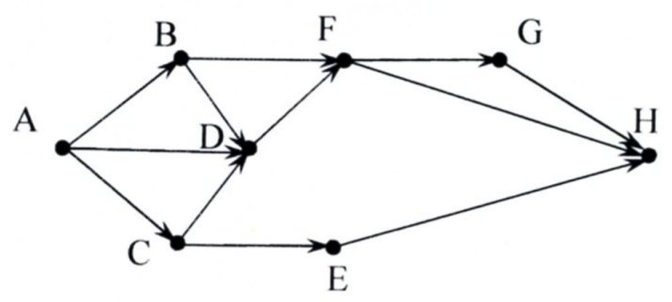
\includegraphics[width=0.95\textwidth]{graph.png}
                \end{center}
            \end{column}
        \end{columns}
        \begin{outline}
            \1 Например:
                \2 Граф дорог, соединяющих города
                \2 Граф компьютерной сети
                \2 Граф зависимостей модулей в процессе компиляции
                \2 Дерево --- подвид графа
            \1 Есть куча известных алгоритмов на графах, позволяющих узнать о них очень многое
        \end{outline}
    \end{frame}

    \begin{frame}
        \frametitle{Определения}
        \begin{outline}
            \1 Ориентированный граф $G$ --- пара из множества вершин $V$ и множества дуг (или рёбер) $E$, где $E$ --- упорядоченная пара вершин $(v, w)$
                \2 $E$ --- бинарное отношение над множеством вершин
                \2 $v$ называется началом, $w$ --- концом дуги
                \2 Дуги вида $(v, v)$ называются петлями
            \1 Путём в орграфе называется последовательность вершин, для которых существуют дуги из предыдущей в следующую
                \2 Длина пути --- количество дуг, составляющих путь
                \2 Путь называется простым, если все вершины на нём, за исключением, быть может, первой и последней, различны
                \2 Цикл --- это простой путь длины не менее 1, который начинается и заканчивается в одной вершине
                \2 Граф без циклов называется ациклическим
        \end{outline}
    \end{frame}

    \begin{frame}
        \frametitle{Ещё определения}
        \begin{outline}
            \1 Неориентированный граф --- это ориентированный граф, у которого для каждого ребра $(v, w)$ существует противоположное ребро $(w, v)$
                \2 то есть отношение $E$ симметрично
            \1 Если $e = (u,v) \in E$, то вершины $u$ и $v$ называются смежными в $G$, а ребро $e$ и эти вершины называются инцидентными
            \1 Степенью вершины в неориентированном графе называется число смежных с ней вершин
                \2 Вершина степени 0 называется изолированной
            \1 Граф может быть помеченным (или взвешенным) – каждой вершине и/или дуге сопоставлена некоторая метка (число, строка и т.д.)
        \end{outline}
    \end{frame}

    \begin{frame}
        \frametitle{Матрица смежности}
        \begin{columns}
            \begin{column}{0.5\textwidth}
                \begin{outline}
                    \1 Для графа из $n$ вершин матрица смежности --- матрица размера $n$ на $n$, где в строке $i$ и столбце $j$ стоит 1 (или true), если есть дуга из $i$ в $j$
                        \2 Для неориентированного графа матрица симметрична относительно главной диагонали
                        \2 Для взвешенного графа вместо 1 стоит вес дуги
                    \1 Занимает $O(n^2)$ памяти, проверка наличия дуги и определение веса --- за константное время
                \end{outline}
            \end{column}
            \begin{column}{0.5\textwidth}
                \begin{center}
                    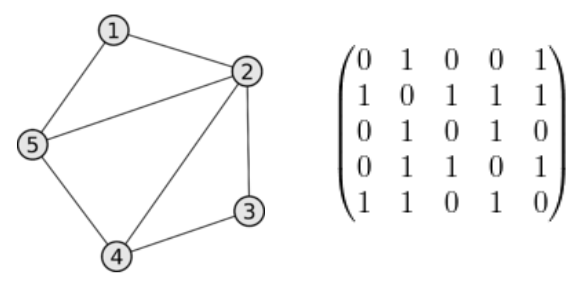
\includegraphics[width=0.95\textwidth]{adjacency-matrix.png}
                \end{center}
            \end{column}
        \end{columns}
    \end{frame}

    \begin{frame}
        \frametitle{Матрица инцидентности}
        \begin{columns}
            \begin{column}{0.5\textwidth}
                \begin{outline}
                    \1 Для графа из $n$ вершин и $m$ ребёр матрица инцидентности --- матрица размера $m$ на $n$, где строка соответствует вершине, а столбец ребру
                        \2 Для ориентированного графа в ячейке $(i, j)$ стоит 1, если ребро $i$ выходит из вершины $j$, и -1, если входит
                        \2 Для неориентированного графа в ячейке $(i, j)$ стоит 1, если ребро $i$ инцидентно вершине $j$
                        \2 Нужно специальное значение для петель
                \end{outline}
            \end{column}
            \begin{column}{0.5\textwidth}
                \begin{center}
                    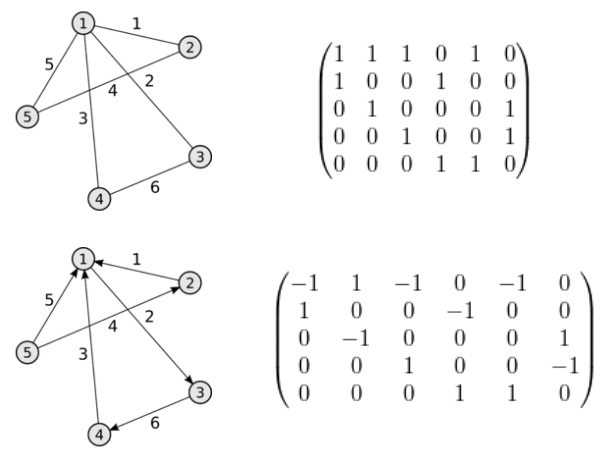
\includegraphics[width=0.95\textwidth]{incidence-matrix.png}
                \end{center}
            \end{column}
        \end{columns}
    \end{frame}

    \begin{frame}
        \frametitle{Матрица инцидентности, свойства}
        \begin{outline}
            \1 В каждом столбце только два элемента ненулевые (1, если петля)
            \1 Для неориентированного графа сумма элементов в столбце равна 2, в строке --- степени вершины
            \1 Требует $O(m * n)$ памяти для хранения
            \1 Проверка наличия ребра между двумя вершинами --- за $O(m)$
            \1 Поиск инцидентных ребру вершин --- за $O(n)$, проверка на инцидентность --- за $O(1)$
        \end{outline}
    \end{frame}

    \begin{frame}
        \frametitle{Список смежности}
        \begin{columns}
            \begin{column}{0.65\textwidth}
                \begin{outline}
                    \1 Для каждой вершины хранится список вершин, смежных с данной
                        \2 Как правило, списки лежат в массиве длины $n$
                        \2 Вместе с номером смежной вершины в списке может лежать вес ребра
                    \1 Требует $O(m + n)$ памяти для хранения
                    \1 Проверка наличия ребра между двумя вершинами --- $O(m)$
                        \2 Если в графе мало рёбер, в среднем $O(1)$
                    \1 Несколько сложнее в реализации
                \end{outline}
            \end{column}
            \begin{column}{0.35\textwidth}
                \begin{center}
                    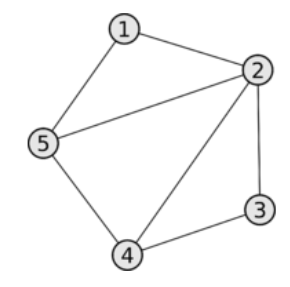
\includegraphics[width=0.95\textwidth]{adjacency-list.png}
                \end{center}
                1: 2, 5 \linebreak
                2: 1, 5, 4, 3 \linebreak
                3: 2, 4 \linebreak
                4: 5, 2, 3 \linebreak
                5: 1, 2, 4
            \end{column}
        \end{columns}
    \end{frame}

    \begin{frame}
        \frametitle{Достижимость}
        \begin{outline}
            \1 Вершина $w$ называется достижимой из вершины $v$, если $v = w$ или в $G$ есть путь от $v$ в $w$
                \2 Рефлексивное и транзитивное замыкание отношения $E$
                \2 Если $E$ симметрично, то достижимость --- отношение эквивалентности
                \2 Классы эквивалентности по отношению достижимости называются компонентами связности
                \2 Для ориентированных графов эквивалентность --- отношение взаимной достижимости
            \1 Проверка на достижимость --- обходы графа в глубину или ширину, алгоритм Уоршелла
        \end{outline}
    \end{frame}

    \begin{frame}
        \frametitle{Обход в глубину}
        \begin{columns}
            \begin{column}{0.5\textwidth}
                \begin{outline}
                    \1 Посещаем вершину
                    \1 Рекурсивно обходим все смежные ей вершины, в которых мы ещё не были
                        \2 Нужно множество (или битовая шкала) посещённых вершин, проще всего передавать как параметр в рекурсивный вызов
                    \1 Можно нерекурсивно, тогда нам потребуется стек рассматриваемых вершин
                        \2 И множество посещённых
                \end{outline}
            \end{column}
            \begin{column}{0.5\textwidth}
                \begin{center}
                    
\includegraphics[width=0.95\textwidth]{dfs.png}
                \end{center}
            \end{column}
        \end{columns}
    \end{frame}

    \begin{frame}
        \frametitle{Обход в ширину}
        \begin{columns}
            \begin{column}{0.7\textwidth}
                \begin{outline}
                    \1 То же, что и обход в глубину, но вместо стека рассматриваемых вершин --- очередь
                    \1 На каждой итерации берём из очереди вершину, посещаем её и кладём в очередь все смежные вершины, в которых мы ещё не были
                        \2 Тоже требуется множество непосещённых вершин
                    \1 Если знаем, что цель недалеко, обход в ширину эффективнее
                    \1 Обход в глубину зато строит глубинное остовное дерево (на самом деле, глубинный остовный лес)
                \end{outline}
            \end{column}
            \begin{column}{0.3\textwidth}
                \begin{center}
                    
\includegraphics[width=0.95\textwidth]{bfs.png}
                \end{center}
            \end{column}
        \end{columns}
    \end{frame}

    \begin{frame}
        \frametitle{Проверка графа на ацикличность}
        \begin{columns}
            \begin{column}{0.7\textwidth}
                \begin{outline}
                    \1 Остовное дерево графа --- подграф, содержащий все вершины графа и являющийся деревом
                        \2 То есть не содержащий циклов, даже если рассматривать граф как неориентированный
                    \1 Глубинное остовное дерево --- путь алгоритма поиска в глубину по графу
                    \1 Обратная дуга --- дуга, не принадлежащая остовному дереву, ведущая от потомка к предку
                        \2 Если обратных дуг нет, в графе нет циклов
                    \1 Посещая вершину, красим её в серый, выходя из её поддерева --- в чёрный
                    \1 Если дуга ведёт в серую вершину, мы нашли цикл
                \end{outline}
            \end{column}
            \begin{column}{0.3\textwidth}
                \begin{center}
                    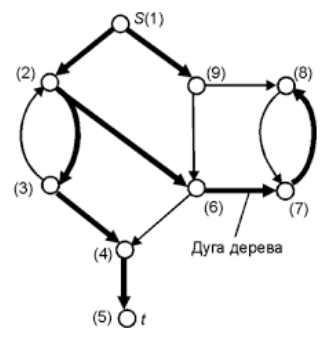
\includegraphics[width=0.95\textwidth]{check-for-acyclicity.png}
                \end{center}
            \end{column}
        \end{columns}
    \end{frame}

    \begin{frame}
        \frametitle{Задача поиска кратчайшего пути в графе}
        \begin{columns}
            \begin{column}{0.65\textwidth}
                \begin{outline}
                    \1 Дан взвешенный ориентированный граф $G = (V, E)$ с неотрицательными весами дуг
                    \1 Одна вершина $s \in V$ помечена как стартовая
                    \1 Задача --- найти кратчайшие пути от стартовой вершины до всех остальных вершин
                        \2 Длина пути определяется как сумма весов дуг, составляющих путь
                    \1 Парадокс изобретателя --- иногда проще решить более общую задачу и получить из неё решение частной задачи, чем решать частную
                        \2 Знание целевой вершины поиск кратчайшего пути не упрощает
                \end{outline}
            \end{column}
            \begin{column}{0.35\textwidth}
                \begin{center}
                    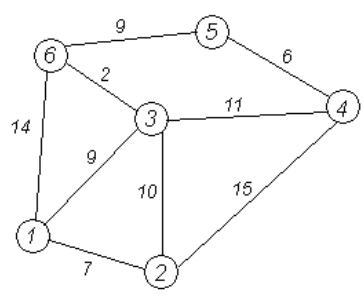
\includegraphics[width=0.95\textwidth]{shortest-path.png}
                \end{center}
            \end{column}
        \end{columns}
    \end{frame}

    \begin{frame}
        \frametitle{Алгоритм Дейкстры}
        Поиск в ширину, где мы запоминаем длину кратчайшего пути в посещённой вершине, обновляя её, если нашли лучше
        \begin{center}
            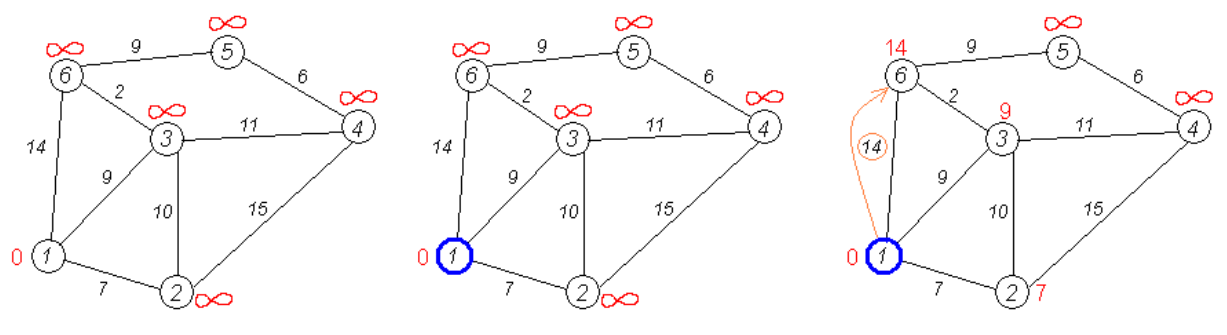
\includegraphics[width=0.95\textwidth]{dijkstra1.png}
        \end{center}
    \end{frame}

    \begin{frame}
        \frametitle{Алгоритм Дейкстры, пример, продолжение}
        Когда все соседи вершины посещены, посчитанная для неё длина пути окончательна и минимальна, выкидываем её из рассмотрения
        \begin{center}
            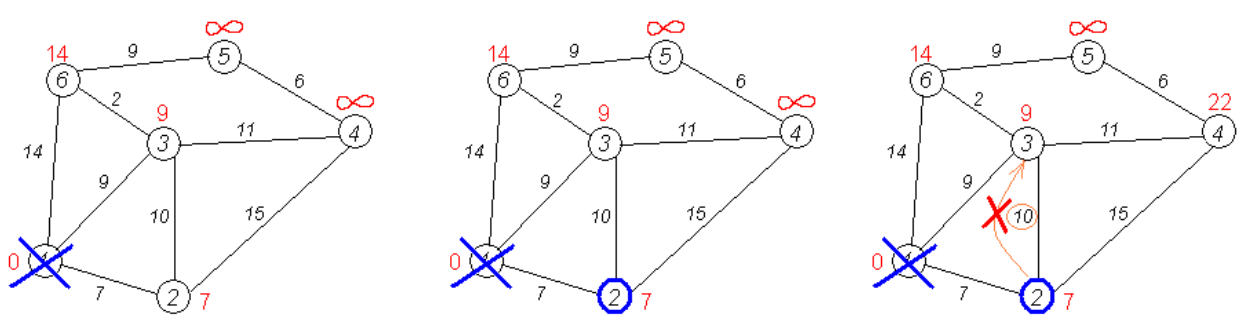
\includegraphics[width=0.95\textwidth]{dijkstra2.png}
        \end{center}
    \end{frame}

    \begin{frame}
        \frametitle{Алгоритм Дейкстры, пример, продолжение (2)}
        Продолжаем, пока не посетили все вершины (правда, бывают несвязные графы)
        \begin{center}
            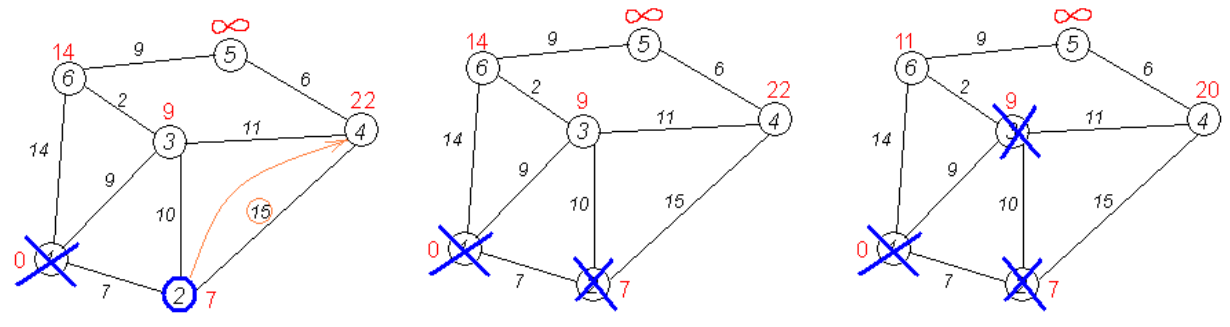
\includegraphics[width=0.95\textwidth]{dijkstra3.png}
        \end{center}
    \end{frame}

    \begin{frame}[fragile]
        \frametitle{Алгоритм Дейкстры, псевдокод}
        \begin{scriptsize}
            \begin{algorithm}[H]
                \DontPrintSemicolon
                \For{$v \in V$}{
                    $d[v] \gets \infty$\;
                    $used[v] \gets false$\;
                }

                $d[s] \gets 0$\;

                \For{$i \in V$}{
                    $v \gets null$\;
                    \For{$j \in V$}{
                        \If{$!used[j]\ and\ (v == null\ or\ d[j] < d[v])$}{
                            $v \gets j$\;
                        }
                    }
                    \If{$d[v] == \infty$}{
                        $break$\;
                    }

                    $used[v] \gets true$\;
                    \For{$e \in $исходящие из v рёбра}{
                        \If{$d[v] + e.len < d[e.to]$}{
                            $d[e.to] \gets d[v] + e.len$\;
                        }
                    }
                }
            \end{algorithm}
        \end{scriptsize}
    \end{frame}

    \begin{frame}
        \frametitle{Тонкости реализации}
        \begin{outline}
            \1 Иногда надо знать не длину пути, а сам путь
                \2 Тогда помимо массива длин $d$ полезно иметь массив родителей $p$, такой что $p[v] = u$, если мы пришли кратчайшим путём в $v$ из $u$
                \2 Обновляем этот массив там же, где мы обновляем $d$
            \1 Множество used можно представлять битовой шкалой, или, если вершин много, множеством на двоичных деревьях или хеш-таблицах
            \1 Поиск ближайшей вершины из множества нерассмотренных можно хранить в очереди с приоритетами, тогда просматривать всё $V$ будет не надо (можно обойтись $O(log(n)$)
                \2 Как --- кучей (вспомните heapsort)
            \1 Трудоёмкость наивной реализации --- $O(n^2 + m)$, с кучей --- $O(n * log(n) + m * log(n))$
        \end{outline}
    \end{frame}

    \begin{frame}
        \frametitle{Почему работает}
        \begin{columns}
            \begin{column}{0.65\textwidth}
                \begin{outline}
                    \1 По индукции
                        \2 На первом шаге $d(s) = 0$, расстояние до неё кратчайшее
                        \2 Для $n$ шагов всё ок, на $n + 1$-м выбрана для добавления вершина $v$. Покажем, что посчитанный для неё сейчас путь --- кратчайший.
                        \2 Если это не так, существует непросмотренная вершина $u$ на кратчайшем пути, $d(v) >= d(u)$, потому что веса путей неотрицательны
                        \2 Но тогда $u$ была бы добавлена раньше, поскольку на каждом шагу выбирается ближайшая к стартовой из непросмотренных вершин
                    \1 Пример жадного алгоритма
                \end{outline}
            \end{column}
            \begin{column}{0.35\textwidth}
                \begin{center}
                    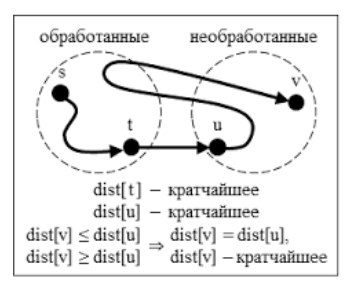
\includegraphics[width=0.95\textwidth]{why-works.png}
                \end{center}
            \end{column}
        \end{columns}
    \end{frame}

    \begin{frame}[fragile]
        \frametitle{Алгоритм Флойда}
        \begin{outline}
            \1 Считает кратчайший путь из каждой вершины в каждую
            \1 Над матрицей смежности выполняется $n$ итераций, на $k$-й итерации $A[i,j]$ содержит значение наименьшей длины путей из вершины $i$ в вершину $j$, которые не проходят через вершины с номером, большим $k$:
            \begin{footnotesize}
                \begin{minted}{pascal}
for k = 1 to n
    for i = 1 to n
        for j = 1 to n
            W[i, j] = min(W[i, j], W[i, k] + W[k, j])
                \end{minted}
            \end{footnotesize}
            \1 Трудоёмкость --- $O(n^3)$
                \2 Зато очень просто реализуется
            \1 Сам кратчайший путь --- заводим матрицу $P$, такую, что на каждой итерации $P[i, j] = k$, дальше рекурсивно восстанавливаем путь по $P[i, k]$ и $P[k, j]$
        \end{outline}
    \end{frame}

    \begin{frame}[fragile]
        \frametitle{Алгоритм Уоршелла}
        \begin{footnotesize}
            \begin{minted}{pascal}
for k = 1 to n
    for i = 1 to n
        for j = 1 to n
            A[i, j] = A[i, j] or (A[i, k]  and A[k, j])
            \end{minted}
        \end{footnotesize}
        \begin{outline}
            \1 Чаще эти два алгоритма называют алгоритмом Флойда-Уоршелла, хотя они разработаны независимо (причём, за 3 года и до Флойда, и до Уоршелла, Бернардом Роем)
            \1 Строит транзитивное замыкание отношения $E$
                \2 Легко искать компоненты связности неориентированного графа
        \end{outline}
    \end{frame}

    \begin{frame}
        \frametitle{Графы и математика}
        \begin{outline}
            \1 Любой граф задаёт бинарное отношение над некоторым множеством
                \2 Ну он и есть бинарное отношение $E$, да
            \1 Ациклический орграф задаёт отношение строгого частичного порядка:
                \2 Антирефлексивность: $\forall x \neg xRx$
                \2 Транзитивность: $\forall x,y,z: xRy \cap yRz \rightarrow xRz$
                \2 Пример: отношения ``больше'' и ``меньше'' на множестве вещественных чисел, отношение строгого включения множеств
            \1 Топологическая сортировка множества $V$ относительно отношения частичного порядка $R$ --- построение последовательности $v_1$, $v_2$, …, $v_n$: 
            $\forall i,j \in 1..n v_i, v_j \in V$ и $v_iRv_j$ или $(v_i, v_j) \not\in R$
                \2 Например, сортировка графа зависимостей файлов при сборке
                \2 Делается поиском в глубину (глубинная остовная нумерация)
        \end{outline}
    \end{frame}

    \begin{frame}
        \frametitle{Доклады}
        \begin{enumerate}
            \item Алгоритм Кнута-Морриса-Пратта
            \item Алгоритм Бойера-Мура
            \item Алгоритм Рабина-Карпа
            \item Алгоритм A*
            \item Визуализация графа пакетом GraphViz
            \item Фильтр Блума
            \item Исключения в C (longjmp)
            \item Длинная арифметика в GMP
            \item Список с пропусками (Skip list)
            \item GNU Readline
        \end{enumerate}
        Доклады через две недели
    \end{frame}

\end{document}